\chapter{Belove nejednakosti}

\section{Postavka problema i izvo{\dj}enje nejednakosti}
Bel je u nadi da će iskristalisati nejasnu sliku EPR paradoksa osmislio eksperiment u kojem bi osa mjerenja spina čestice bila proizvoljna i nezavisna od druge (anti)čestice, za razliku od postavke eksperimenta EPRB (slika \ref{fig:bell_exp_figure}).

Recimo da su u pitanju elektron i pozitron dobijeni raspadom $\pi^0$ mezona.
Za tako arbitraran pravac mjerenja možemo detektovati spin "gore" ili "dole", $1$ ili $-1$ (u jedinicama $\hbar/2$) respektivno.
Umjesto posmatranja pojedinačnog rezultata mjerenja za elektron i pozitron, posmatramo proizvod ta dva rezultata, koji može uzimati vrijednosti $\pm1$.
Neka je srednja vrijednost ovih proizvoda $P(\vec{a},\vec{b})$.
Ako dozvolimo da su $\vec{a}$ i $\vec{b}$ paralelni, proizvod je uvijek $-1$ jer su spinovi u 100\% slučajeva opozitni, dakle

\begin{equation}
    \vec{a} = \vec{b} \implies P(\vec{a}, \vec{a}) = -1.
\end{equation}
Istom logikom, ako su ti pravci antiparalelni, svaki proizvod će biti $+1$, dakle

\begin{equation}
    \vec{a} = -\vec{b} \implies P(\vec{a}, -\vec{a}) = 1.
\end{equation}
Za proizvoljne pravce $\vec{a}$ i $\vec{b}$ standardna kvantna mehanika predvi\dj a (vidjeti Dodatak):

\begin{equation}
    P(\vec{a}, \vec{b}) = - \vec{a} \cdot \vec{b}. \label{eq:srednja_vrijednost_proizvoda}
\end{equation}

\begin{figure}[H]
    \centering
    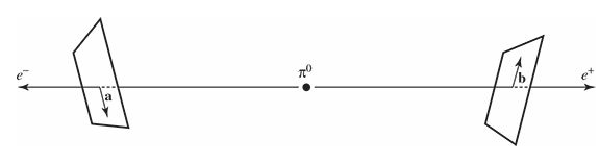
\includegraphics[width=0.75\textwidth]{figures/bell_scheme.eps}
    \caption{Belova postavka misaonog eksperimenta sa osama mjerenja koje mogu biti
        u proizvoljnim pravcima.}
    \label{fig:bell_exp_figure}
\end{figure}

Po\dj imo sada od pretpostavke da zaista postoji neka skrivena varijabla $\lambda$ koja omogućuje kompletniji opis stanja.
Pretpostavimo dalje da je ishod mjerenja elektrona nezavisan od orijentacije detektora pozitrona  $\vec{b}$. Naime, tu orijentaciju bi eksperimentator koji se nalazi kod detektora pozitrona mogao izabrati neposredno prije nego što je izvršeno mjerenje elektrona, dakle prekasno da bi se bilo koja informacija koja se prenosi brzinom manjom od brzine svjetlosti vratila do detektora elektrona. Ova pretpostavka u Belovoj verziji EPRB eksperimenta je u suštini {\it{pretpostavka o lokalnosti}}.
Tada postoje neke funkcije $A(\vec{a}, \lambda)$ i $B(\vec{b}, \lambda)$, koje zavise od skrivene varijable $\lambda$ i određuju rezultate mjerenja elektrona, odnosno pozitrona.
Ove funkcije mogu da imaju samo vrijednosti $+1$ i $-1$, dakle 

\begin{equation}
    A(\vec{a}, \lambda) = \pm 1, \quad B(\vec{b}, \lambda) = \pm 1.
\end{equation}
Kada su detektori poravnati, rezultati su za sve vrijednosti $\lambda$ savršeno antikorelisani, tj.

\begin{equation}
    A(\vec{a}, \lambda) = -B(\vec{b}, \lambda).
\end{equation}

Srednja vrijednost proizvoda pojedinačnih mjerenja je data sa

\begin{equation}
    P(\vec{a}, \vec{b}) = \int \rho (\lambda) A(\vec{a}, \lambda) B(\vec{b}, \lambda) d\lambda
\end{equation}
gdje smo sa $\rho (\lambda)$ označili gustinu vjerovatnoće skrivene varijable.
Ako posmatramo slučaj u kojem su detektori postavljeni u pravcima koji su međusobno paralelni, izmjerićemo uvijek suprotne spinove pa važi

\begin{equation}
    A(\vec{m}, \lambda) = - B(\vec{m}, \lambda).
\end{equation}
Srednja vrijednost proizvoda sada može da se napiše kao

\begin{equation}
    P(\vec{a}, \vec{b}) = - \int \rho (\lambda) A(\vec{a}, \lambda) A(\vec{b}, \lambda) d\lambda.
\end{equation}
Za bilo koji drugi jedinični vektor $\vec{c}$ važi takođe

\begin{equation}
    P(\vec{a}, \vec{c}) = - \int \rho (\lambda) A(\vec{a}, \lambda) A(\vec{c}, \lambda) d\lambda.
\end{equation}
Ako oduzmemo ove dvije jednačine dobijamo

\begin{equation}
    P(\vec{a}, \vec{b}) - P(\vec{a}, \vec{c})  = - \int \rho (\lambda) [A(\vec{a}, \lambda) A(\vec{b}, \lambda) - A(\vec{a}, \lambda) A(\vec{c}, \lambda) ] d\lambda.
\end{equation}
Zbog toga što je

\begin{equation}
    [A(\vec{b}, \lambda)]^2 = 1
\end{equation}
za proizvoljan vektor $\vec{b}$, drugi član u integrandu možemo pomnožiti sa takvom "jedinicom", pa dobijemo

\begin{equation}
    P(\vec{a}, \vec{b}) - P(\vec{a}, \vec{c})  = - \int \rho (\lambda) \left\{A(\vec{a}, \lambda) A(\vec{b}, \lambda) - A(\vec{a}, \lambda) A(\vec{c}, \lambda)[A(\vec{b}, \lambda)]^2 \right\}d\lambda.
\end{equation}
Jednostavnim izvlačenjem ispred zagrade dobijemo

\begin{equation}
    P(\vec{a}, \vec{b}) - P(\vec{a}, \vec{c})  = - \int \rho (\lambda) A(\vec{a}, \lambda) A(\vec{b}, \lambda) [1- A(\vec{c}, \lambda) A(\vec{b}, \lambda) ] d\lambda.
\end{equation}
Uzmimo sada apsolutnu vrijednost ovog izraza:

\begin{equation}
    \left|{P(\vec{a}, \vec{b}) - P(\vec{a}, \vec{c})}\right| =  \left| \int  \rho (\lambda) A(\vec{a}, \lambda) A(\vec{b}, \lambda) [1- A(\vec{c}, \lambda) A(\vec{b}, \lambda)  ] d\lambda \right|.
\end{equation}
Pošto funkcije $A$ i $B$ uzimaju vrijednosti $\pm 1$ lako je vidjeti da je

\begin{equation}
    \left|A(\vec{a}, \lambda) A(\vec{b}, \lambda)\right| = 1.
\end{equation}

Analizirajmo sada član koji je preostao:

\begin{equation}
    \rho (\lambda)[1 - A(\vec{c}, \lambda) A(\vec{b}, \lambda) ].
\end{equation}
S obzirom da je $\rho(\lambda)$ gustina vjerovatnoće, kao takva funkcija mora biti ne-negativna tako da za taj član važi

\begin{equation}
    \rho(\lambda) \ge0 , \quad \forall \lambda.
\end{equation}
Proizvod $A(\vec{c}, \lambda) A(\vec{b}, \lambda)$ može imati vrijednosti $\pm 1$ tako da je

\begin{equation}
    1 - A(\vec{c}, \lambda) A(\vec{b}, \lambda) \ge 0 , \quad \forall \lambda.
\end{equation}
Dakle,

\begin{equation}
    \rho (\lambda)[1 - A(\vec{c}, \lambda) A(\vec{b}, \lambda) ] \ge 0, \quad \forall \lambda.
\end{equation}
Slijedi:


\begin{equation}
    \left|{P(\vec{a}, \vec{b}) - P(\vec{a}, \vec{c})}\right| \le  \int  \rho (\lambda)  [1- A(\vec{c}, \lambda) A(\vec{b}, \lambda)  ]  d\lambda = \underbrace{\int \rho(\lambda)d\lambda}_{1} + P(\vec{c}, \vec{b}).
\end{equation}
Konačno dobijemo Belovu nejednakost

\begin{equation}
    \left|{P(\vec{a}, \vec{b}) - P(\vec{a}, \vec{c})}\right| \le 1 +  P(\vec{c}, \vec{b}).
\end{equation}
Rezultat važi za bilo koju teoriju skrivenih varijabli, jer je $\rho(\lambda)$ proizvoljna funkcija raspodjele.

\section{Narušenje Belovih nejednakosti i implikacije}

Konstruišimo sada jednostavan primjer kojim možemo pokazati da, ako standardna kvantna mehanika važi,  dolazi do narušavanja Belovih nejednakosti. Na slici
su prikazana tri pravca u kojima možemo izvršiti mjerenje.

Želimo izračunati srednju vrijednost proizvoda izmjerenih spinova po formuli \eqref{eq:srednja_vrijednost_proizvoda}, koju smo dobili u okviru standardne kvantne mehanike (Dodatak).
Ako sa $\theta$ ozna\v cimo ugao me\dj u pravcima $\vec{a}$ i $\vec{b}$, onda se ova formula mo\v ze napisati u obliku
\begin{equation}
    P(\vec{a},\vec{b}) = -\mathrm{cos} \:\! \theta.
\end{equation}\\


% \begin{minipage}{0.6\textwidth}
% Your TikZ picture code here
\begin{tikzpicture}[scale=3, shift={(10,10)}]
    \def\arrowlength{1.5}

    % Arrow at 90 degrees
    \draw[->] (0,0) -- (\arrowlength,0) node[midway, below] {$\overrightarrow{b}$};

    % Arrow at 90 degrees
    \draw[->] (0,0) -- (0,\arrowlength) node[midway, left] {$\overrightarrow{a}$};

    \def\arrowlength{2}

    % Arrow at 45 degrees
    \draw[->] (0,0) -- (45:\arrowlength) node[midway, above, right] {$\overrightarrow{c}$};

    % draw arc
    \draw (0,0) -- (0.5,0) arc (0:45:0.5) -- cycle;
    \node at (0.3,0.15) {45\textdegree};
\end{tikzpicture}
\captionof{figure}{Detektori postavljeni sa relativnim uglovima od $45^\degree$ i $90^\degree$.}
\label{fig:detectors_with_chosen_angles}
% \end{minipage}

Ako izaberemo da ugao između pravaca $\vec{a}$ i $\vec{b}$ bude $90^\degree$, a uglovi ime\dj u pravaca $\vec{a}$ i $\vec{c}$, odnosno $\vec{b}$ i $\vec{c}$, po $45^\degree$ (slika: \ref{fig:detectors_with_chosen_angles}), Belova nejednakost glasi:
\begin{equation*}
    | \mathrm{cos}(90^\degree) - \mathrm{cos}(45^\degree)|\le 1 + \mathrm{cos}(45^\degree).
\end{equation*}
Vidimo da ova nejednakost nije istinita, te zaključujemo da, ako se srednje vrijednosti $P(\vec{a},\vec{b})$, $P(\vec{b},\vec{c})$, $P(\vec{a},\vec{c})$ računaju prema kvantnoj mehanici (tj. po formuli (\ref{eq:srednja_vrijednost_proizvoda})), Belove nejednakosti su narušene.

Sa Belovom modifikacijom EPR paradoks dokazuje nešto mnogo radikalnije nego što su njegovi autori zamislili:
Ako su u pravu, onda ne samo da je kvantna mehanika nepotpuna, već je i pogrešna.
S druge strane, ako je kvantna mehanika u pravu, onda nas nijedna teorija skrivenih varijabli neće spasiti od nelokalnosti koju je Ajnštajn smatrao apsurdnom.
Odavde proizilazi da bi realan eksperiment, kojim bi se utvrdilo da li su Belove nejednakosti narušene ili važe, razriješio dilemu - standardna kvantna mehanika ili neka lokalna teorija skrivenih varijabli.
